\chapter{实验技术 I：安全、测量与分离}\label{ch:b1:lab-techniques-1}

两名学生对同一批阿司匹林进行重结晶，并在同一加热台上测定其
熔点。一人读得 \qty{134}{\celsius}，另一人
读得 \qty{136}{\celsius}。两人的结果是否矛盾？产物是否纯净？
这些问题仅凭两个数字无法回答：测量值只有
附带不确定度才有意义，比较则须依据
某种规则。本章汇总本学年的实验实践内容：如何
读懂台面上各种物质的危害，如何表述测量值
及其不确定度并与另一结果比较，以及有机实验室
的经典操作——萃取、过滤、重结晶、蒸馏——如何将
产物与周围物质分离，
再检验其是否纯净。

\begin{recall}
由分子间作用力判断溶解性与互溶性，区分极性溶剂与非极性溶剂
（见\cref{ch:b1:intermolecular-forces-solvents}）；滴定管、移液管
及滴定终点（见\cref{ch:b1:titration-methods}）。
第 1 册（十年级）中已引入液–液萃取、
重结晶、薄层色谱法和合成的产率；
本章则为它们给出具体的数值。
\end{recall}

\begin{omfigure}
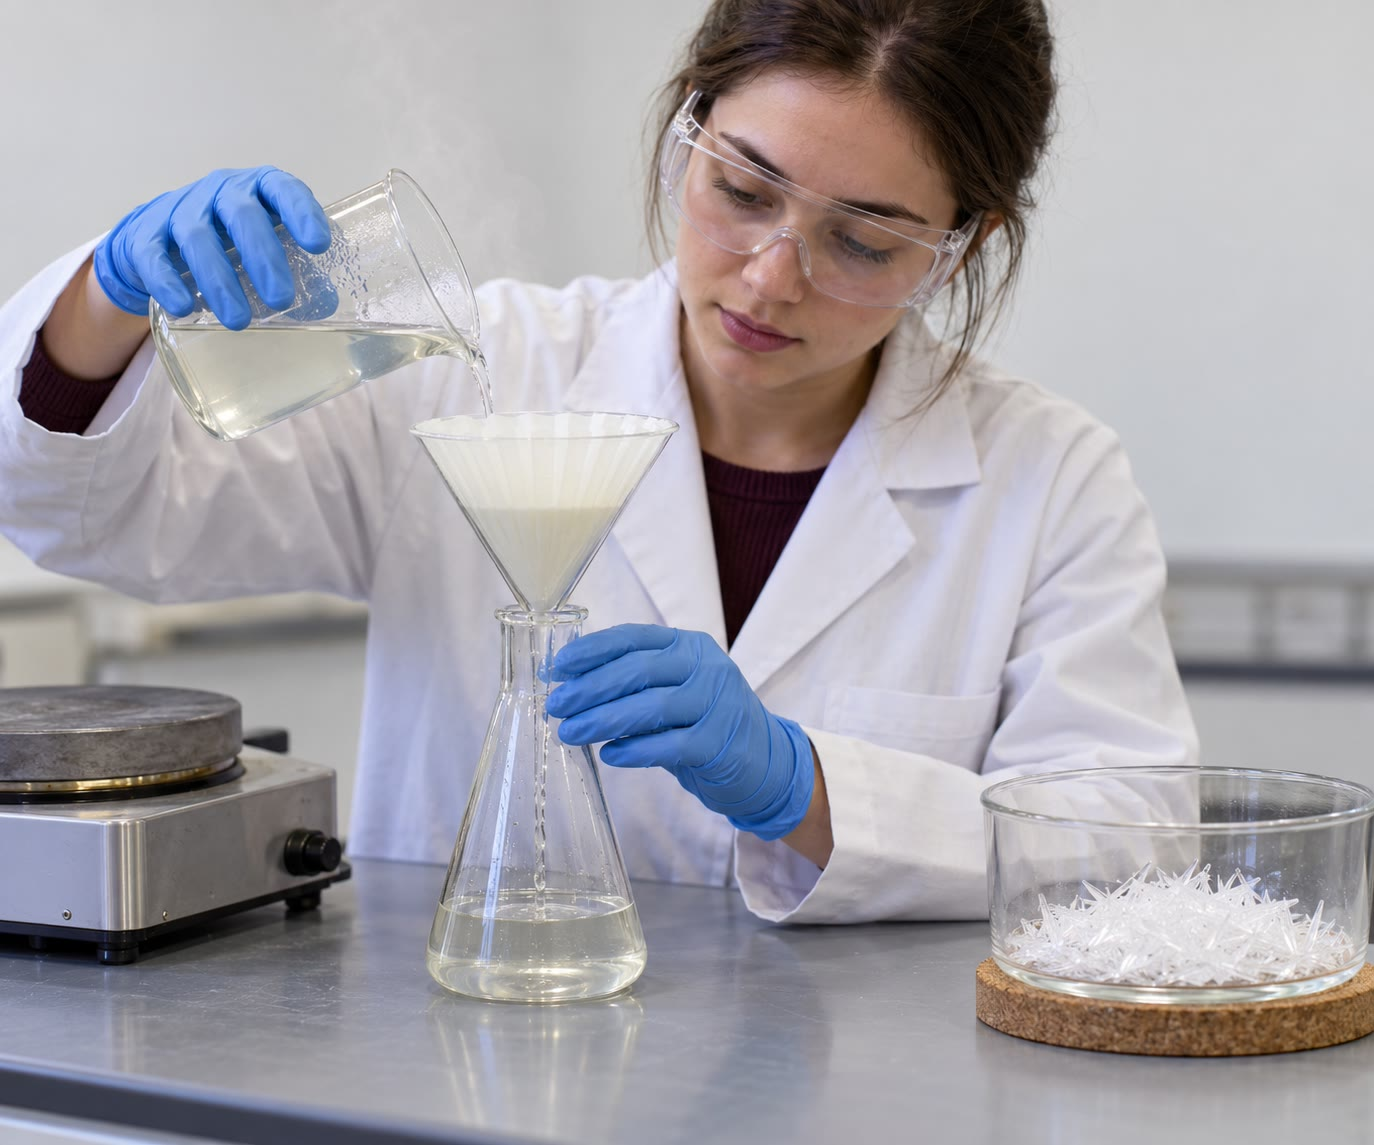
\includegraphics[width=0.5\linewidth]{images/book2/ai/b1-29-recrystallisation.jpg}

{\small 重结晶过程中的热过滤：护目镜、手套和实验服；热溶液
通过一张折叠滤纸，
滤纸截留不溶性杂质，重结晶得到的针状产物
放在右侧的培养皿中。}
\end{omfigure}

\section{危害及其标签}

\begin{definition}[危害与风险]\label{def:b1:lab-techniques-1:hazard}
\emph{危害}\index{危害}是物质（或某种情形）的固有性质，
可能造成伤害，如易燃性、腐蚀性、毒性。\emph{风险}\index{风险}是
在给定使用条件下实际发生伤害的可能性及其严重程度，
取决于危害本身以及接触情况
（用量、浓度、时长、途径、
防护措施）。
\end{definition}

危害无法在不改变物质的情况下改变；风险则可以通过
控制接触情况来降低：减少用量、改用更稀的溶液、
使用通风橱、戴手套和护目镜，或改用危害较小的试剂
完成同一操作。

\begin{definition}[GHS 标签]\label{def:b1:lab-techniques-1:ghs}
化学品的标签遵循全球化学品统一分类和标签制度（GHS）。
\begin{itemize}
  \item \emph{危险象形图}\index{危险象形图}是置于带红色边框的
        白色菱形上的黑色图形，共九种，\texttt{GHS01}
        至\texttt{GHS09}。
  \item \emph{信号词}\index{信号词}对较严重的危害类别为\emph{危险}，
        对较轻者为\emph{警告}；
        标签只标注一个，即较严重者。
  \item \emph{危险说明}\index{危险说明}是描述危害的标准化用语，
        以 H 加三位数字编码：
        H2xx 为物理危害，H3xx 为健康危害，H4xx 为
        环境危害。
  \item \emph{防范说明}\index{防范说明}是以 P 加三位数字编码，
        给出应采取措施的标准用语：P1xx 为一般性，
        P2xx 为预防，P3xx 为响应，P4xx 为储存，P5xx 为处置。
  \item \emph{安全技术说明书}\index{安全技术说明书}是供应商随产品提供的
        文件，采用标准章节结构，依次为标识、危害、组成、
        急救、消防措施、操作与储存、
        接触控制与个人防护、理化性质、
        稳定性、毒性、
        处置与运输。
\end{itemize}
\end{definition}

\begin{omfigure}
\setlength{\tabcolsep}{5pt}
\begin{tabular}{ccccc}
\begin{tabular}[t]{@{}c@{}}\ghs[1.25cm]{GHS01}\\[2pt]\footnotesize GHS01\\\footnotesize 爆炸物\end{tabular} &
\begin{tabular}[t]{@{}c@{}}\ghs[1.25cm]{GHS02}\\[2pt]\footnotesize GHS02\\\footnotesize 易燃\end{tabular} &
\begin{tabular}[t]{@{}c@{}}\ghs[1.25cm]{GHS03}\\[2pt]\footnotesize GHS03\\\footnotesize 氧化性\end{tabular} &
\begin{tabular}[t]{@{}c@{}}\ghs[1.25cm]{GHS04}\\[2pt]\footnotesize GHS04\\\footnotesize 加压气体\end{tabular} &
\begin{tabular}[t]{@{}c@{}}\ghs[1.25cm]{GHS05}\\[2pt]\footnotesize GHS05\\\footnotesize 腐蚀性\end{tabular} \\[8pt]
\begin{tabular}[t]{@{}c@{}}\ghs[1.25cm]{GHS06}\\[2pt]\footnotesize GHS06\\\footnotesize 急性毒性\end{tabular} &
\begin{tabular}[t]{@{}c@{}}\ghs[1.25cm]{GHS07}\\[2pt]\footnotesize GHS07\\\footnotesize 有害、刺激性\end{tabular} &
\begin{tabular}[t]{@{}c@{}}\ghs[1.25cm]{GHS08}\\[2pt]\footnotesize GHS08\\\footnotesize 健康危害\end{tabular} &
\begin{tabular}[t]{@{}c@{}}\ghs[1.25cm]{GHS09}\\[2pt]\footnotesize GHS09\\\footnotesize 环境\end{tabular} & \\
\end{tabular}

\smallskip
{\small 九种 GHS 象形图：爆炸弹、火焰、火焰在圆圈上方、
气瓶、腐蚀、骷髅与交叉骨、感叹号、健康
危害（长期效应：致癌、突变、生殖毒性、
呼吸道致敏、吸入危害）和环境危害。}
% ledger: ghspic:GHS01, ghspic:GHS02, ghspic:GHS03, ghspic:GHS04,
% ghspic:GHS05, ghspic:GHS06, ghspic:GHS07, ghspic:GHS08, ghspic:GHS09
\end{omfigure}

\begin{example}[读懂乙醇的标签]
一瓶乙醇标注有象形图 GHS02 和 GHS07，信号词
为\emph{危险}，并标注危险说明 H225（高度易燃的液体和蒸气，
属物理危害，其类别要求使用\emph{危险}）和 H319
（造成严重眼刺激，属健康危害，单独出现时为\emph{警告}）。
其防范说明包括 P210（远离热源、火花和明火；禁止吸烟）、
P233（容器保持密闭）、P280（戴手套和护目镜）、
P305+P351+P338（若入眼：小心
用水冲洗数分钟，取出隐形眼镜，继续
冲洗）、P403+P235（储存于通风良好处，保持低温）。
实际后果：使用乙醇的台面上不得有明火，
佩戴护目镜，瓶子须密闭。
\end{example}
% ledger: ghs:ethanol, hstat:H225, hstat:H319, pstat:P210, pstat:P233,
% pstat:P280, pstat:P305+P351+P338, pstat:P403+P235

\begin{method}[根据安全技术说明书准备实验]\label{met:b1:lab-techniques-1:read-sds}
对每种使用或生成的物质：
\begin{enumerate}
  \item 查看其危险象形图、信号词和 H 说明（安全技术说明书第 2 节），
        并记下物理危害（火灾、压强、
        反应性），与健康和环境危害分开记录；
  \item 对每项操作（称量、加热、转移、过滤），
        估计接触量：用量、状态（易挥发液体或细粉末会进入肺部）、
        持续时间；
  \item 选择防护措施：以危害较小的试剂替代、
        缩小规模、使用通风橱，再采取个人防护（P2xx
        说明）；
  \item 规划事故应对（P3xx：眼睛、皮肤、误食、
        火灾）措施，以及每类废弃物的去向（P5xx）。
\end{enumerate}
\end{method}

\begin{inthelab}[废弃物]
默认情况下，任何东西都不得倒入水槽。有机溶剂分别收集于
两个容器：卤代溶剂（二氯甲烷、三氯甲烷）和
非卤代溶剂（乙醇、丙酮、环己烷、乙酸乙酯），因
两者处理方式不同；酸、碱水溶液
需中和后方可弃置；重金属离子溶液（铬、
铜、银）各有专用容器；破碎的玻璃和受污染的
固体与普通垃圾分开存放。说明 P273“避免
释放到环境中”印在标签上，提醒人们废液
容器而非水槽，才是实验的终点。
% ledger: pstat:P273
\end{inthelab}

\section{测量与不确定度}

测量值从来不是被测量的精确值：重复
测量，结果会略有变化；读取刻度时，
末位数字只是估计。不确定度说明真值可能合理地
偏离测量值的范围有多大。

\begin{definition}[测量不确定度]\label{def:b1:lab-techniques-1:uncertainty}
\begin{itemize}
  \item 称\emph{测量不确定度}\index{测量不确定度}
        为一个参数，表征
        可合理归因于被测量的数值的分散程度。
  \item 称\emph{标准不确定度}\index{标准不确定度} $u(x)$
        为以标准差表示的该不确定度。
  \item \emph{A 类评定}\index{A 类评定}得到 $u$，方法是
        对一系列重复测量作统计分析；
        \emph{B 类评定}\index{B 类评定}则以其他任何方式得到它，如
        仪器的刻度、
        制造商给出的容差、校准证书、
        表列数值的位数。
  \item \emph{扩展不确定度}\index{扩展不确定度}
        $U = k\,u$ 为标准不确定度乘以包含因子
        $k$，通常取 $k = 2$；对正态分布，
        区间 $x \pm 2u$ 包含真值的概率为
        约 \qty{95}{\percent}。
  \item 称\emph{相对不确定度}\index{相对不确定度}为
        $u(x)/|x|$，常以百分数表示。
\end{itemize}
\end{definition}

\begin{proposition}[A 类评定]\label{prop:b1:lab-techniques-1:type-a}
若对同一量进行了 $n$ 次独立测量 $x_1, \dots, x_n$，
则最佳估计为其均值 $\bar x$；实验标准
差为
\[
  s = \sqrt{\frac{1}{n-1} \sum_{i=1}^{n} (x_i - \bar x)^2},
\]
而均值的标准不确定度为 $u(\bar x) = s/\sqrt{n}$。
\end{proposition}
\begin{proof}[\omnameProof]
\emph{在本阶段不加证明地承认}；重复测量的统计处理，
包括 $n$ 较小时所用的学生系数，
在本科二年级分册中讨论。
\end{proof}

\begin{omfigure}
\begin{tikzpicture}
\begin{axis}[width=7.4cm, height=5cm, xlabel={终点体积（\unit{mL}）},
  ylabel={读数个数}, ymin=0, ymax=8.5, xmin=12.2, xmax=12.7,
  xtick={12.2,12.3,12.4,12.5,12.6,12.7},
  xticklabel style={/pgf/number format/fixed, /pgf/number format/precision=1},
  axis lines=left, every axis plot/.append style={line join=round}]
  \addplot[ybar, bar width=0.045, fill=omDef!35, draw=omDef!80!black]
    table[x=V, y=count] {figdata/out/bachelor-1-type-a-uncertainty-a.dat}; % 横坐标 V，纵坐标 count 为读数个数
  \addplot[omThm, thick, smooth]
    table[x=V, y=g] {figdata/out/bachelor-1-type-a-uncertainty-b.dat};
  \draw[omProp, thick, <->] (axis cs:12.384,7.6) -- (axis cs:12.526,7.6);
  \node[omProp, font=\small, above] at (axis cs:12.455,7.6) {$\bar V \pm s$};
\end{axis}
\end{tikzpicture}\hspace{0.6cm}%
\begin{tikzpicture}
\begin{axis}[width=5.6cm, height=5cm, xlabel={$x - x_0$}, ylabel={密度},
  ymin=0, ymax=0.8, xmin=-1.6, xmax=1.6, xtick={-1,0,1},
  xticklabels={$-a$, $0$, $a$}, ytick={0.5}, yticklabels={$\frac{1}{2a}$},
  axis lines=left]
  \addplot[omDef!80!black, thick, fill=omDef!25] coordinates
    {(-1,0) (-1,0.5) (1,0.5) (1,0)} \closedcycle;
  \draw[omProp, thick, <->] (axis cs:-0.577,0.62) -- (axis cs:0.577,0.62);
  \node[omProp, font=\small, above] at (axis cs:0,0.62) {$\pm a/\sqrt3$};
\end{axis}
\end{tikzpicture}

{\small 左图：同一滴定终点的二十次读数（示意数据），
读数精确到 \qty{0.05}{mL}，并绘出正态分布曲线，
其均值 $\bar V = \qty{12.455}{mL}$，标准差 $s = \qty{0.071}{mL}$。
右图：B 类评定的矩形分布，对应仅知其取值
位于 $x_0 - a$ 与 $x_0 + a$ 之间的情形；其标准差为
$a/\sqrt3$。}
\end{omfigure}

\begin{example}[二十个滴定终点]
对图中二十个读数，$\bar V = \qty{12.455}{mL}$，
$s = \qty{0.071}{mL}$ 且 $u(\bar V) = 0.071/\sqrt{20} = \qty{0.016}{mL}$。
单次读数的不确定度约为 $s$；二十次读数的平均值的不确定度约为
$s/\sqrt{20}$，约小四倍半。结果为
$V = \qty{12.46}{mL}$，扩展不确定度为 $U = 2u = \qty{0.03}{mL}$。
\end{example}

\begin{proposition}[矩形分布的 B 类评定]\label{prop:b1:lab-techniques-1:type-b}
若某量所知的仅是它以相等的
概率落在 $x_0 - a$ 与 $x_0 + a$ 之间的任一处，则其标准
不确定度为
\[
  u = \frac{a}{\sqrt3}.
\]
\end{proposition}
\begin{proof}
概率密度为 $1/(2a)$，只在 $[x_0 - a, x_0 + a]$ 上取值，
其余处为零；由对称性，其均值为 $x_0$，方差为
\[
  u^2 = \int_{x_0-a}^{x_0+a} (x - x_0)^2 \frac{\mathrm{d}x}{2a}
      = \frac{1}{2a} \left[\frac{t^3}{3}\right]_{-a}^{a}
      = \frac{1}{2a}\cdot\frac{2a^3}{3} = \frac{a^2}{3}. \qedhere
\]
\end{proof}

\begin{example}[一次读数与容差]
刻度间隔为 \qty{0.1}{mL} 的滴定管，读数精确到半格：
读数与所记录值的差在 $\pm\qty{0.05}{mL}$ 之内，因此
$u = 0.05/\sqrt3 = \qty{0.029}{mL}$。一支 \qty{20}{mL} 移液管，
其制造商标称容差为 $\pm\qty{0.03}{mL}$，其放出体积的
标准不确定度为 $u = 0.03/\sqrt3 = \qty{0.017}{mL}$。一个表列值写作
\qty{135}{\celsius}，其误差为 $\pm\qty{0.5}{\celsius}$：$u = \qty{0.29}{\celsius}$。
\end{example}

\begin{proposition}[不确定度的合成]\label{prop:b1:lab-techniques-1:combine}
对相互独立的量：若 $y = x_1 + x_2$ 或 $y = x_1 - x_2$，则
$u(y)^2 = u(x_1)^2 + u(x_2)^2$；若 $y = x_1 x_2$ 或 $y = x_1/x_2$，则
\[
  \left(\frac{u(y)}{y}\right)^2 = \left(\frac{u(x_1)}{x_1}\right)^2
  + \left(\frac{u(x_2)}{x_2}\right)^2 .
\]
同一量的若干不确定度来源（A 类分量与 B 类分量）
亦按同样方式、以平方和合成。
\end{proposition}
\admitted

相加的是平方，而非不确定度本身：两个独立误差
很少会以满幅度朝同一方向作用。滴定所得体积
是两次滴定管读数之差，因此其读数的不确定度为
$\sqrt2 \times \qty{0.029}{mL} = \qty{0.041}{mL}$；另外，一个较大的不确定度来源
往往主导其余来源，改进应
着眼于此。一般规则涉及偏导数，留待
本科二年级分册讨论。

\begin{method}[结果的报告]\label{met:b1:lab-techniques-1:report-result}
\begin{enumerate}
  \item 列出不确定度来源；将每个量都评定为标准
        不确定度（A 类由一组数据得出，B 类由半宽
        按 $a/\sqrt3$ 评定）。
  \item 将它们以平方和合成（见\cref{prop:b1:lab-techniques-1:combine}）。
  \item 给出扩展不确定度 $U = 2u$，取一位或两位
        有效数字，并将结果值取至相同小数位，记作
        $x = (\text{值} \pm U)$ 单位，包含因子 $k = 2$。
\end{enumerate}
\end{method}

\begin{definition}[归一化偏差]\label{def:b1:lab-techniques-1:z-score}
同一量的两个独立值之间的\emph{归一化偏差}\index{归一化偏差}（或 $z$ 分数），
记两值为 $x_1$ 与 $x_2$，标准不确定度分别为
$u_1$ 与 $u_2$，则
\[
  z = \frac{|x_1 - x_2|}{\sqrt{u_1^2 + u_2^2}} .
\]
当 $z \le 2$ 时，称两值相容；测量值
与参考值相容，同样以此为判据。
\end{definition}

\begin{example}[两位学生]
开篇所述的两个熔点，\qty{134}{\celsius} 与
\qty{136}{\celsius}，分别测得，标准不确定度均为
\qty{0.8}{\celsius}（来自读数与实验台校准）。于是
$z = 2/\sqrt{0.8^2 + 0.8^2} = 1.8 \le 2$，两位学生的结果一致。其平均值
\qty{135}{\celsius}，亦与阿司匹林的表列熔点
（快速加热下测得的 \qty{135}{\celsius}）相容。表中值只给到单位，其
$u = 0.5/\sqrt3 = \qty{0.29}{\celsius}$，故单次读数
（$u = \qty{0.8}{\celsius}$）只要与之相差
不超过 $2\sqrt{0.8^2 + 0.29^2} = \qty{1.7}{\celsius}$，即与之相容：读数
低于约 \qty{133}{\celsius} 时，则提示产物不纯。
\end{example}
% ledger: mp:aspirin

\section{分离}

\begin{definition}[分配系数]\label{def:b1:lab-techniques-1:partition-coefficient}
溶质 A 在平衡时分配于两种不互溶的
溶剂（有机相与水相）之间，其
浓度之比
\[
  K = \frac{[\mathrm{A}]_{\mathrm{org}}}{[\mathrm{A}]_{\mathrm{aq}}}
\]
在一定温度下、对稀溶液为常数，
称为 A 在
两溶剂之间的\emph{分配系数}\index{分配系数}。
\end{definition}

\begin{proposition}[多次萃取优于一次萃取]\label{prop:b1:lab-techniques-1:multiple-extractions}
对体积为 $V_a$ 的水溶液进行 $n$ 次萃取，每次
均用体积为 $V_o$ 的新鲜有机溶剂。水相中残留的
A 的分数为
\[
  f_n = \left(1 + K \frac{V_o}{V_a}\right)^{-n}.
\]
溶剂总量一定时，分 $n$ 小份萃取优于
一次大体积萃取。
\end{proposition}
\begin{proof}
设 $m$ 为一次萃取前水相中 A 的量，
$m'$ 为萃取后的量。平衡时有机相含 $m - m'$，且
$K = \dfrac{(m - m')/V_o}{m'/V_a}$，故 $m - m' = K\dfrac{V_o}{V_a} m'$，且
$m' = m\big/\bigl(1 + K V_o/V_a\bigr)$。每次萃取都使剩余量
乘以同一因子；经 $n$ 次萃取后，$f_n$ 为
该因子的 $n$ 次方。若总体积 $V$ 分为 $n$ 份，每份 $V/n$，
$\ln f_n = -n \ln(1 + KV/(nV_a))$；由于 $\ln(1+t)/t$ 随 $t$ 增大而减小，
$n \ln(1 + t/n)$ 随 $n$ 增大（$t = KV/V_a > 0$），于是 $f_n$
随之减小，趋于极限 $\mathrm{e}^{-KV/V_a}$。
\end{proof}

\begin{example}[一份还是三份]
某溶质 $K = 4$，自 \qty{100}{mL} 水中，用
\qty{60}{mL} 乙酸乙酯萃取。一次萃取时，
$f_1 = 1/(1 + 4 \times 0.6) = 0.29$：\qty{71}{\percent} 被萃取。若分
三次，每次 \qty{20}{mL}，$f_3 = (1 + 4 \times 0.2)^{-3} = 0.17$：
\qty{83}{\percent}。乙酸乙酯（$\rho = \qty{0.90}{g/cm^3}$）为
分液漏斗中的上层；二氯甲烷
（$\rho = \qty{1.33}{g/cm^3}$）则为下层。
\end{example}
% ledger: rho:ethyl-acetate, rho:CH2Cl2, rho:water

过滤可将固体与液体分离。在重力作用下，
通过漏斗中的折叠滤纸，截留热溶液中的不溶性杂质；该热溶液
在过滤过程中不可冷却（即热过滤，见本章开头的照片）。
减压时，用布氏漏斗装在抽滤瓶上（如第 1 册所示），
可迅速收集固体并使其几近干燥；
固体在滤器上用少量冷
溶剂洗涤。

\begin{definition}[重结晶]\label{def:b1:lab-techniques-1:recrystallisation}
\emph{重结晶}\index{重结晶}提纯固体：将固体
溶于最少量的热溶剂中，该溶剂对其热时溶解度大、
冷时溶解度小，然后冷却使其结晶；
杂质或仍溶解于冷溶剂中（即母液），
或因不溶而预先经热过滤除去。
\end{definition}

\begin{method}[固体重结晶]\label{met:b1:lab-techniques-1:recrystallise}
\begin{enumerate}
  \item 选择溶剂：产物热时溶解度大，
        冷时溶解度小；可溶杂质即使冷时也可溶；
        与产物不反应，沸点低于产物的熔点；
        也可用两种互溶溶剂（乙醇与水）的混合物，
        以适配产物。
  \item 将粗固体溶于最少量的沸腾溶剂中，
        分小份加入；若溶剂易挥发或易燃，则
        加热回流。
  \item 若仍有不溶性杂质，则热过滤。
  \item 让溶液缓慢冷却，再置于冰中：缓慢冷却
        可得较大、较纯的晶体，晶体所包裹的母液较少。
  \item 减压过滤，用少量冰冷的
        溶剂洗涤，干燥，称重；检验纯度（熔点、薄层色谱）。
\end{enumerate}
\end{method}

\begin{example}[纯度的代价]
阿司匹林在 \qty{25}{\celsius} 水中的溶解度约为 \qty{3.3}{g/L}，
在 \qty{37}{\celsius} 时为 \qty{10}{g/L}，接近沸点时
则大得多。若 \qty{40}{mL} 母液与 \qty{10}{mL} 洗涤水
在 \qty{25}{\celsius} 时流出滤器，它们约带走
$\qty{0.050}{L} \times \qty{3.3}{g/L} = \qty{0.17}{g}$ 的阿司匹林，
无论其纯度如何。超出最少用量的每一毫升溶剂，都会损失产率。
\end{example}
% ledger: sol:aspirin-25, sol:aspirin-37

提纯液体，或分离沸点相差较大的两种液体，均可用
\emph{简单蒸馏}：将混合物加热沸腾，
蒸气中较易挥发组分的含量较高，经冷凝后
收集。侧臂处的温度即为馏出蒸气的温度；
温度保持恒定时，即有纯净物馏出。
沸点相近的液体需用分馏，即在烧瓶与
蒸馏头之间加装分馏柱，并借助
本科二年级分册中的液–气相图来处理。

\begin{omfigure}
\begin{tikzpicture}[font=\small, scale=0.95]
  \pic[transform shape] at (0,0) {heatingmantle};
  \pic[transform shape] at (0,0) {rbflask={0.45}{orange!25}};
  \foreach \x/\y in {-0.35/0.25,0.05/0.18,0.35/0.3}
    \fill[black!55] (\x,\y) circle (0.06);
  \pic[transform shape] (s) at (0,3.0) {stillhead};
  \pic[transform shape] at ($(s-top)+(0,-0.75)$) {thermometer};
  \pic[transform shape, rotate=-20] (c) at (s-arm) {liebig={3.4}};
  \coordinate (cend) at ($(s-arm)+(-20:3.4)$);
  \pic[transform shape] (a) at (cend) {adapter};
  \pic[transform shape] at ($(a-tip)+(0,-2.4)$) {erlenmeyer={0.22}{orange!12}};
  \draw[<-, omProp, thick] (0.12,3.72) -- (-1.4,4.4) node[left, text=black,
    align=right] {温度计球泡 \\与侧管平齐};
  \draw[<-, omProp, thick] ($(s-arm)+(-20:0.65)+(0.65,0.65)$) -- ++(0.2,0.9)
    node[above, text=black] {冷却水出};
  \draw[<-, omProp, thick] ($(s-arm)+(-20:2.7)+(-0.2,-0.6)$) -- ++(0.05,-0.9)
    node[below, text=black] {冷却水入};
  \draw[<-, omProp, thick] (-0.3,0.27) -- (-2.2,0.7) node[left, text=black]
    {沸石};
  \draw[<-, omProp, thick] (1.35,-0.6) -- (2.3,-1.1) node[right, text=black]
    {加热套};
  \draw[<-, omProp, thick] ($(a-tip)+(0.75,-2.0)$) -- ++(1.0,0.2)
    node[right, text=black] {馏出液};
\end{tikzpicture}

{\small 简单蒸馏。温度计示数为进入冷凝器的
蒸气温度；冷却水从冷凝器下端进入，
使夹套始终充满水；沸石可防止
剧烈暴沸；接收端与大气相通。}
\end{omfigure}

\begin{safety}{\ghs[5mm]{GHS02}}
蒸馏装置决不可封闭：受热时，密闭体系会爆裂。
沸石应加入冷的液体中，切勿加入
已经加热的液体中（否则可能立即暴沸）。易燃的馏出液
应远离明火收集，必要时将接收器置于冰中。
\end{safety}

\section{鉴定与检验纯度}

\begin{definition}[比移值]\label{def:b1:lab-techniques-1:retention-factor}
在薄层色谱法（TLC）中，将样品斑点点在
涂有固定相（硅胶）的薄板下端附近的基线上；
薄板置于盛有少量洗脱剂的密闭槽中，洗脱剂
借毛细作用沿涂层上升，并使各组分以
不同速率移动。某组分的\emph{比移值}\index{比移值}
为：
\[
  R_f = \frac{\text{斑点移动的距离}}
             {\text{洗脱剂前沿移动的距离}},
\]
两者均自基线量起；$0 \le R_f \le 1$，对于给定的
固定相、洗脱剂及温度，它表征该组分。
\end{definition}

在极性硅胶上，极性较强的组分比极性较弱的组分被吸附得更牢，
其 $R_f$ 较小；极性更强的洗脱剂使每个斑点
移动得更远。同一块板上两个组分的 $R_f$ 相同，仍可能有所不同；
而两个不同的 $R_f$ 则证明二者不同。纯净的产物只给出
一个斑点。

\begin{omfigure}
\begin{tikzpicture}[font=\small, scale=1.7]
  \pic[transform shape] at (0,0) {tlcplate};
  \draw[omDef!80!black, densely dashed, line width=0.5pt] (-0.7,2.7) -- (0.7,2.7);
  \foreach \x in {-0.4,0,0.4} \fill[black!60] (\x,0.4) circle (0.025);
  \fill[omThm!70] (-0.4,{0.4+0.30*2.3}) ellipse (0.09 and 0.06);
  \fill[omDef!70] (0,{0.4+0.65*2.3}) ellipse (0.09 and 0.06);
  \fill[omThm!70] (0.4,{0.4+0.30*2.3}) ellipse (0.09 and 0.06);
  \fill[omDef!70] (0.4,{0.4+0.65*2.3}) ellipse (0.09 and 0.06);
  \node[below] at (-0.4,0) {A}; \node[below] at (0,0) {B};
  \node[below] at (0.4,0) {M};
  \draw[omProp, thick, |<->|] (0.95,0.4) -- (0.95,{0.4+0.65*2.3})
    node[midway, right] {$d_{\mathrm{B}}$};
  \draw[omProp, thick, |<->|] (1.55,0.4) -- (1.55,2.7)
    node[midway, right] {$d_{\mathrm{front}}$};
  \draw[omProp, thick, |<->|] (-0.95,0.4) -- (-0.95,{0.4+0.30*2.3})
    node[midway, left] {$d_{\mathrm{A}}$};
  \node[right, align=left, font=\footnotesize] at (0.75,2.85) {洗脱剂前沿};
  \draw[omProp, thick, <-] (-0.6,0.4) -- (-1.2,0.05) node[left, text=black, font=\footnotesize] {基线};
\end{tikzpicture}

{\small 显影后的薄层色谱板：参照物 A 和 B，以及混合物 M，
点样于基线上。$R_f(\mathrm{A}) = d_{\mathrm{A}}/d_{\mathrm{front}}
= 0.30$，$R_f(\mathrm{B}) = 0.65$；混合物 M
显示两个斑点，位于相同高度。}
\end{omfigure}

\begin{method}[进行薄层色谱]\label{met:b1:lab-techniques-1:tlc}
\begin{enumerate}
  \item 用铅笔在距底边约 \qty{1}{cm} 处画出基线，并在其上
        点上样品与参照物稀溶液的小斑点，
        使各斑点并排排列。
  \item 在槽中（基线以下）加入几毫米深的洗脱剂，
        盖紧，使槽内气氛饱和；将薄板直立放入其中。
  \item 当前沿距顶端约 \qty{1}{cm} 时取出薄板，
        立即标出前沿，晾干。
  \item 显出无色斑点（紫外灯照射荧光板，
        碘蒸气熏显或显色剂处理），并用铅笔圈出。
  \item 测量各斑点距基线的距离，计算各 $R_f$；
        在同一块板上将样品与参照物进行比较。
\end{enumerate}
\end{method}

\begin{omfigure}
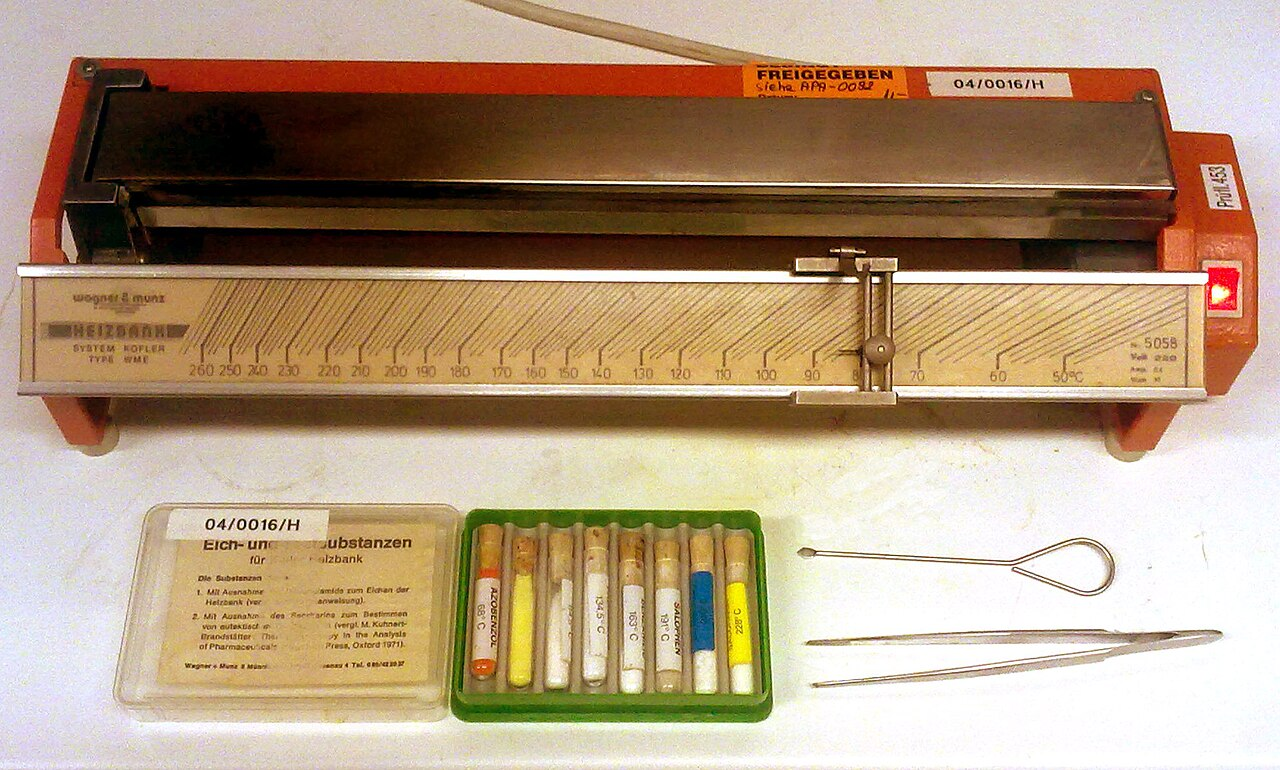
\includegraphics[width=0.62\linewidth]{images/book2/kofler-bench.jpg}

{\small 加热台（科夫勒热台）：金属条一端受热，
沿条形成温度梯度；将固体撒在条上，
越过一条清晰的界线即熔化，由指针在刻度上读数。盒中
装有已知熔点的参照物，用于校准热台。
照片：HBR，CC BY-SA 3.0，维基共享资源。}
\end{omfigure}

\begin{method}[在加热台上测定熔点]\label{met:b1:lab-techniques-1:melting-point}
\begin{enumerate}
  \item 提前充分开启热台：温度梯度需要一段时间
        才能稳定。
  \item 用一种纯的参照物校准热台，其熔点应接近
        预期值，撒在金属条上；调节指针，使
        刻度上的读数与其熔点在界线处相符。
  \item 从冷端向热端撒上少量干燥样品的晶体；
        用药匙来回推动，
        并将指针置于固体立即熔化的界限处。
  \item 读数，重复测定，清洁金属条；取读数的平均值，
        并给出不确定度（\cref{met:b1:lab-techniques-1:report-result}）。
\end{enumerate}
\end{method}

纯的晶体物质在其熔点处熔化得很清晰；不纯的物质
开始熔化的温度更低，并在一个温度范围内熔化，
这是因为杂质降低了固液共存的温度
（其原因在于溶剂的化学势因溶质而降低，
详见本科二年级分册）。熔点明显低于
列表值，或熔化范围较宽，因此表明含有杂质；
若数值与列表值在归一化
偏差的意义上相容，则支持该物质为纯净物，但不能由此证明。

\begin{inthelab}[校准热台]
所选参照物的熔点应将预期值夹在其中。乙酰苯胺
熔点为 \qty{114.3}{\celsius}，苯甲酸为
\qty{122.4}{\celsius}，是熔点在
\qty{110}{\celsius} 至 \qty{130}{\celsius} 之间产物的经典标准；若要更好，
可用熔点约 \qty{135}{\celsius} 的阿司匹林作标准。阿司匹林本身在熔化时会分解，
因此其观测熔点取决于加热速度：列表值为
快速加热时的 \qty{135}{\celsius}，这正是热台的加热方式。
% ledger: mp:acetanilide, mp:benzoic, mp:aspirin
\end{inthelab}

液体可借其\emph{折射
率} $n_D$，即真空中光速与光在
液体中的速率之比，用钠的黄色 D 线在规定温度下测得，
（通常为 \qty{20}{\celsius}），精确到小数点后四位。
在 \qty{20}{\celsius} 时，水的 $n_D = 1.333$，乙醇为 1.3611，环己烷为 1.4266。
折射率随温度升高而略有下降，因此仪器
需保持恒温。
% ledger: nD:water, nD:ethanol, nD:cyclohexane

\begin{omfigure}
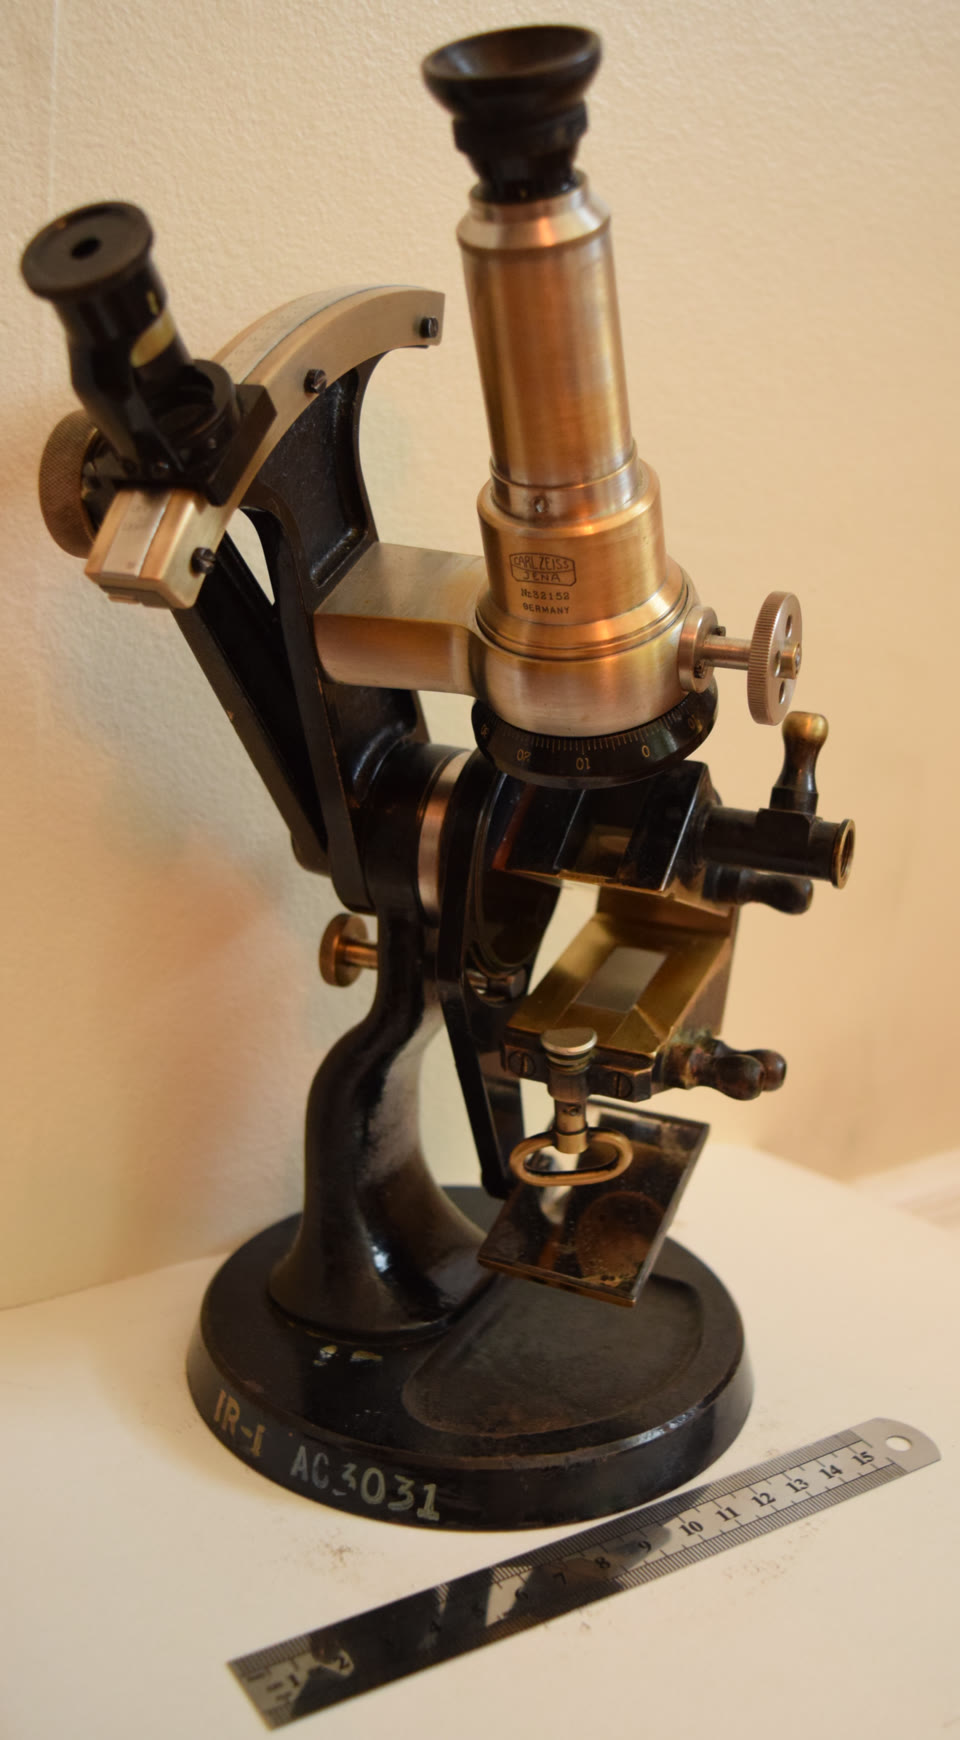
\includegraphics[height=6cm]{images/book2/abbe-refractometer.jpg}

{\small 阿贝折射仪：在两块棱镜之间涂上一滴液体；
目镜中视场一半明亮、一半暗淡，
将明暗界线对准十字线，即可在刻度上读出折射率。
照片：Foreade，CC BY-SA 4.0，维基共享资源。}
\end{omfigure}

\section{练习}

\begin{exercise}[$\star$]\label{exo:b1:lab-techniques-1:1}
一瓶丙酮带有象形图 GHS02 和 GHS07，以及
危险说明 H225、H319 和 H336。其信号词为何？
哪些危险说明描述物理危害，哪些描述健康危害？
列举它们要求采取的两项防范措施。
\end{exercise}

\begin{exercise}[$\star$]\label{exo:b1:lab-techniques-1:2}
判断下列各项所述是“危害”还是“风险”。(a) 浓硫酸会造成严重烧伤。
(b) 在通风橱中戴手套称取 \qty{50}{mg} 有毒粉末，操作者所受暴露很小。
(c) 钠与水反应放出氢气。
(d) 同一溶剂，
在敞口烧杯中加热使用，比在密闭瓶中冷用更危险。
\end{exercise}

\begin{exercise}[$\star$]\label{exo:b1:lab-techniques-1:3}
在一块薄层色谱板上，洗脱剂前沿距基线 \qty{6.0}{cm}；
样品在 \qty{2.1}{cm} 和 \qty{4.2}{cm} 处出现斑点。计算它们的
$R_f$。同板点样的标准品上升至 \qty{4.2}{cm}，
可得出哪些结论，哪些不能得出？
\end{exercise}

\begin{exercise}[$\star$]\label{exo:b1:lab-techniques-1:4}
刻度为每格 \qty{0.1}{mL} 的滴定管，读数估读至半格。
求单次读数的标准不确定度，再求
放出体积（两次读数之差）的标准不确定度。
\end{exercise}

\begin{exercise}[$\star\star$]\label{exo:b1:lab-techniques-1:5}
同一样品五次称量结果分别为 \qty{0.2512}{g}、\qty{0.2508}{g}，
\qty{0.2515}{g}、\qty{0.2510}{g} 和 \qty{0.2505}{g}。求其平均值、
实验标准偏差、平均值的标准不确定度，
并以 $k = 2$ 报告结果。
\end{exercise}

\begin{exercise}[$\star\star$]\label{exo:b1:lab-techniques-1:6}
分配系数为 $K = 3$ 的某溶质，在有机溶剂与
水之间分配。用共 \qty{30}{mL} 溶剂，从 \qty{50}{mL} 水中萃取，
求一次萃取、分两份萃取以及分三份萃取时的萃取分数，
其中两份各 \qty{15}{mL}，三份各 \qty{10}{mL}。
\end{exercise}

\begin{exercise}[$\star\star$]\label{exo:b1:lab-techniques-1:7}
一次滴定给出浓度为 \qty{0.1012}{mol/L}，标准不确定度为
\qty{0.0006}{mol/L}；该溶液的配制浓度为 \qty{0.1000}{mol/L}，
标准不确定度为 \qty{0.0002}{mol/L}。两个值是否
相容？若滴定的不确定度改为
\qty{0.0004}{mol/L}，又如何？
\end{exercise}

\begin{exercise}[$\star\star$]\label{exo:b1:lab-techniques-1:8}
某固体在三种溶剂中的溶解度（示意值，以 \unit{g} 每 \qty{100}{mL} 计）为：
溶剂 P 冷时为 1.5，沸腾时为 2.0；溶剂
Q 冷时为 0.3，沸腾时为 12；溶剂 R 冷时为 9，沸腾时为 25。哪种
溶剂适合重结晶，为何不选另外两种？选用合适溶剂时，
\qty{5.0}{g} 该固体中可回收的最大比例是多少，
若沸腾溶剂用量取最少，
并将混合物冷却？
\end{exercise}

\begin{exercise}[$\star\star$]\label{exo:b1:lab-techniques-1:9}
一种恒温于 \qty{20}{\celsius} 的无色液体，
其 $n_D = 1.3612$。它可能是水、乙醇和环己烷中的哪一种？
为何要注明温度？若折射率为 1.350，则说明什么？
\end{exercise}

\begin{exercise}[$\star\star\star$]\label{exo:b1:lab-techniques-1:10}
利用 \cref{exo:b1:lab-techniques-1:6} 的数据，证明无论
\qty{30}{mL} 溶剂分得多细，溶质至多可被萃取的比例为
$1 - \mathrm{e}^{-KV/V_a}$，并求该值。
分成几份可达到该极限的 \qty{99}{\percent}？
\end{exercise}

\begin{exercise}[$\star\star\star$]\label{exo:b1:lab-techniques-1:11}
已知某量位于 $x_0 - a$ 与 $x_0 + a$ 之间，取值靠近
$x_0$ 的可能性更大：其概率密度为三角形，$(a - |x - x_0|)/a^2$。
验证其已归一化，并证明其标准不确定度为
$a/\sqrt6$。与矩形分布的情形作比较。
\end{exercise}

\begin{exercise}[$\star\star\star$]\label{exo:b1:lab-techniques-1:12}
将 \cref{exo:b1:lab-techniques-1:5} 中的样品
（摩尔质量为 \qty{204.2}{g/mol}，不确定度可忽略）溶于一只
\qty{100.00}{mL} 容量瓶中，其容积的标准不确定度为
\qty{0.06}{mL}。求该溶液的浓度，以及其相对不确定度和
扩展不确定度。
哪一来源占主导？
\end{exercise}

\section{问题：阿司匹林的提纯}

\begin{problem}[{周末问题——合成的危害、粗阿司匹林的
重结晶及其产率、带 A 类与 B 类不确定度的熔点，
以及与表列值的
归一化偏差}]
\label{pb:b1:lab-techniques-1:1}
一名学生将 \qty{2.00}{g} 水杨酸与过量的
乙酸酐加热，制得阿司匹林，再对粗产物进行重结晶。
摩尔质量（\unit{g/mol}）：水杨酸 \ce{C7H6O3} 138.0，阿司匹林
\ce{C9H8O4} 180.0，乙酸酐 \ce{C4H6O3} 102.0。标签：
水杨酸 GHS05、GHS07、H302、H318；乙酸酐 GHS02、
GHS05、GHS06、GHS07、H226、H302、H314、H332；阿司匹林 GHS07、H302。
阿司匹林在水中的溶解度：\qty{25}{\celsius} 时为 \qty{3.3}{g/L}。
阿司匹林的表列熔点（快速加热）：\qty{135}{\celsius}。
% ledger: ghs:salicylic, ghs:acetic-anhydride, ghs:aspirin, sol:aspirin-25,
% mp:aspirin, hstat:H318, hstat:H226, hstat:H314, hstat:H302

\medskip
\noindent\textbf{第一部分——危害。}
\begin{enumerate}
  \item 乙酸酐标签上的每个象形图各表示什么？
  \item 水杨酸标签带有哪一信号词？阿司匹林的
        又是哪一个？
  \item 乙酸酐的危害更为严重。试说明，
        处理 \qty{5}{mL} 该物质时，风险仍可如何降至很低？
  \item 乙酸酐的哪些危险说明要求佩戴护目镜和手套，
        哪些要求使用通风橱并避免明火？
  \item 若一滴乙酸酐溅入眼睛，应立即采取什么措施？
  \item 重结晶的滤液中，水中含有乙酸和少量乙醇，
        它应如何处理？
\end{enumerate}

\noindent\textbf{第二部分——合成与重结晶。}
\begin{enumerate}[resume]
  \item 写出合成反应的方程式，以乙酸
        \ce{C2H4O2} 为副产物，并检查方程式是否配平。
  \item 计算水杨酸的物质的量及阿司匹林的
        理论最大质量。
  \item 粗产物干燥后的质量为 \qty{2.41}{g}。为何不能跳过
        重结晶，尽管产量已达到
        理论最大值的 \qty{92}{\percent}？
  \item 阿司匹林用少量乙醇溶解，再以热水
        补足。为何与接近沸点时相比，\qty{25}{\celsius}下水中的溶解度
        才是起决定作用的性质？
  \item 为何要将粗固体溶于最少量的热溶剂中？
  \item 为何溶液要先缓慢冷却，再置于冰中？
  \item 有 \qty{40}{mL} 在 \qty{25}{\celsius} 下的滤液离开漏斗，
        随后又有 \qty{5}{mL} 洗涤水流出。估算随之
        损失的阿司匹林质量。
  \item 纯净干燥产物质量为 \qty{1.95}{g}。计算产率。
\end{enumerate}

\noindent\textbf{第三部分——熔点。}
\begin{enumerate}[resume]
  \item 实验台上六次读数（事先已校准）分别为 134、135、
        133、135、134 和 \qty{136}{\celsius}。计算其平均值。
  \item 计算实验标准差。
  \item 由此求出平均值的 A 类标准不确定度。
  \item 每次读数精确到最接近的度。计算读数的 B 类
        不确定度。
  \item 实验台的校准保证在
        $\pm\qty{1}{\celsius}$ 以内。计算相应的 B 类
        不确定度，再求合成标准不确定度。
  \item 报告熔点及其扩展不确定度（$k = 2$）。
  \item 一位同学的粗产物在 120 至
        \qty{128}{\celsius} 之间熔化。这说明什么？
\end{enumerate}

\noindent\textbf{第四部分——与参考值比较。}
\begin{enumerate}[resume]
  \item 表中数值精确到个位。该数值隐含的
        标准不确定度为多少？
  \item 薄层色谱板（溶剂前沿 \qty{6.0}{cm}）上，粗产物
        出现位于 \qty{2.3}{cm} 和 \qty{3.3}{cm} 处的斑点，水杨酸在
        \qty{2.3}{cm} 处显示一个斑点，重结晶产物在
        \qty{3.3}{cm} 处显示一个斑点。计算 $R_f$ 值并作出结论。
  \item 为何阿司匹林的熔点与加热速率有关？
  \item 计算测量熔点与表中熔点之间的归一化偏差 $z$，
        并判断二者是否相容。
\end{enumerate}
\end{problem}
